%%% TeX-master: "../main.tex"
% kapitel5.tex
\chapter{Konkret getestete Applikationen}\label{chapter:concretetests}


Dieses Kapitel stellt nun einige Ergebnisse, die mittels des nach dem Konzepts tatsächlich
implementierten vollautomatischen GUI-Crawler und -Tester erzeugt wurden.
Als erstes getestetes Programm dient hierbei eine Enwicklerversion der von der
\textbf{e-Spirit AG} entwickelten Software \textbf{FirstSpirit} 
\footnote{\url{ http://www.e-spirit.com/de/produkt/arbeiten-mit-firstspirit/usability-fuer-redakteure/ }},
Version 5.2 DEV 201. Entwicklerversionen dieser Software enthalten zusätzliche,
dem normalen Nutzer unzugängliche Schaltflächen und Funktionen.

Als zweite Applikation wurde der beliebte Texteditor \textbf{jEdit}
\footnote{\url{ http://www.jedit.org/ }} gewählt. Die dritte ist
die Java-Graphvisualisierungssuite \textbf{yEd}
\footnote{\url{ http://www.yworks.com/products/yed }}.



\section{Resultate FirstSpirit}\label{section:testresults}

Wie in den Graphdarstellungen auf Seiten \pageref{fig:model_firstspirit_notext} und 
\pageref{fig:model_freespirit_06.10.2015} zu sehen ist, enthält diese Version von
FirstSpirit etwa 34 einzigartige Fenster bzw. Zustände. Sie gehen fast alle vom
Hauptfenster des Programms bzw. dem Zustand zu Beginn des Tests aus,
nur einige wenige sind dahingegen tiefer abzweigend. Die Zahl einer im
Laufe eines vollen Durchgangs betätigter Eingabeelemente liegt im Vergleich bei
über 800. Dies legt nahe, dass umfangreiche interne Zustandsänderungen
möglich sind, die nicht direkt in von außen sichtbaren geänderten
Programmzuständen resultieren. Oder auch, dass eine Menge Eingabeelemente
existieren oder als solche erkannt wurden, deren Betätigung kein messbares
Resultat hatte.

Bedenkt man die Natur von FirstSpirit, ist dies keine große Überraschung.
FirstSpirit ist ein Content Management System bzw. CMS, im Grunde also
ein Client bzw. Editor für Webinhalte. Da der Autotester lediglich den Editor testet,
ohne Rücksicht auf die Inhalte nehmen zu wollen oder auch zu können,
hat die Mehrzahl der getätigten Eingaben keinen für das Konzept erkennbaren
Effekt. Änderungen am editierten Projekt haben aber für den Editor durchaus
-- wie auch immer geartete -- langfristige Konsequenzen, und es ist für
einen produktiven Einsatz des Autotesters anzuraten, solche von Seiteneffekten
beeinflussten Daten vor jedem Testdurchlauf wieder auf einen ursprünglichen
Zustand zurückzusetzen.

Nach Dutzenden von Testdurchläufen auf einem nie zurückgesetzten System
ist das von der e-Spirit AG genutzte Beispielprojekt \glqq{}Mithras\grqq{}
erheblich beschädigt. Zufällige Betätigung diverser Löschbefehle hat
Elemente aus dem Projekt entfernt bzw. Verknüpfungen gelöscht, die für
eine korrekte Funktion spezifischer Bestandteile nötig wären. Obwohl
dies natürlich Auswirkungen auf das Testverfahren hat, zeigt sich doch,
dass dennoch in etwa dieselbe Anzahl von Eingabeelementen getestet wird,
die graphische Oberfläche also nicht zwangsläufig auf ein korrekt funktionierendes
geladenes Projekt angewiesen ist, um alle möglichen Eingaben auszuprobieren.

In einer Produktivumgebung würde der Autotester folgendermaßen integriert:
Im Gegensatz zu Unit-Tests mit JUnit können keine festen Maßstäbe angelegt
werden, nach denen eine Version des Quellcodes zulässig ist oder auch nicht.
Korrektheit ist nicht das erklärte oder auch nur erreichbare Ziel.
Der Autotester wäre dementsprechend nicht im regulären automatischen
Build-Prozess enthalten (und diesen irgendwie anhalten oder behindern),
sondern wäre parallel angeordnet und kontinuierlich oder nach Wunsch
Tests durchführen. Man könnte sich z.B. vorstellen, dass eine neue
Programmversion jeweils fünfhundert (die Zahl ist völlig arbiträr) Durchläufe
des Autotesters auslöst und erfahren soll. Jede Instanz des Testprogramms wird
in einem virtualisiertem System gestartet, in das man vorher die
zentral gelagerte Konfigurationsdatei sowie die nötigen Voraussetzungen
kopiert hat -- in diesem Fall wäre dies das FirstSpirit-Programm sowie
die Dateien des Mithras-Projekts.

Die Logdateien und Ergebnis-Graphen jeder Instanz würden dann wieder zentral
gesammelt und könnten dann auf Gemeinsamkeiten und Abweichungen untersucht
werden. Instanzen, die nicht korrekt beendeten, sind natürlich von besonderem
Interesse. FirstSpirit hat eine eigene Schnittstelle, um Fehlerberichte von
aufgetretenen Ausnahmen weiterzureichen. Diese Berichte sowie in den Logdateien
erwähnte Fehlermeldungen könnten dann von Entwicklern genutzt werden, um
Schwachstellen im Code auszumerzen, wenn diese denn tatsächlich vorliegen.
Idealerweise ist es dem Autotester irgendwann unmöglich, Fehlermeldungen
oder Ausnahmen herbeizuführen, da die Entwickler jede ursprünglich 
unvorhergesehene Eingabe oder -sequenz abfangen oder korrekt behandeln.


\begin{sidewaysfigure}
	\centering
	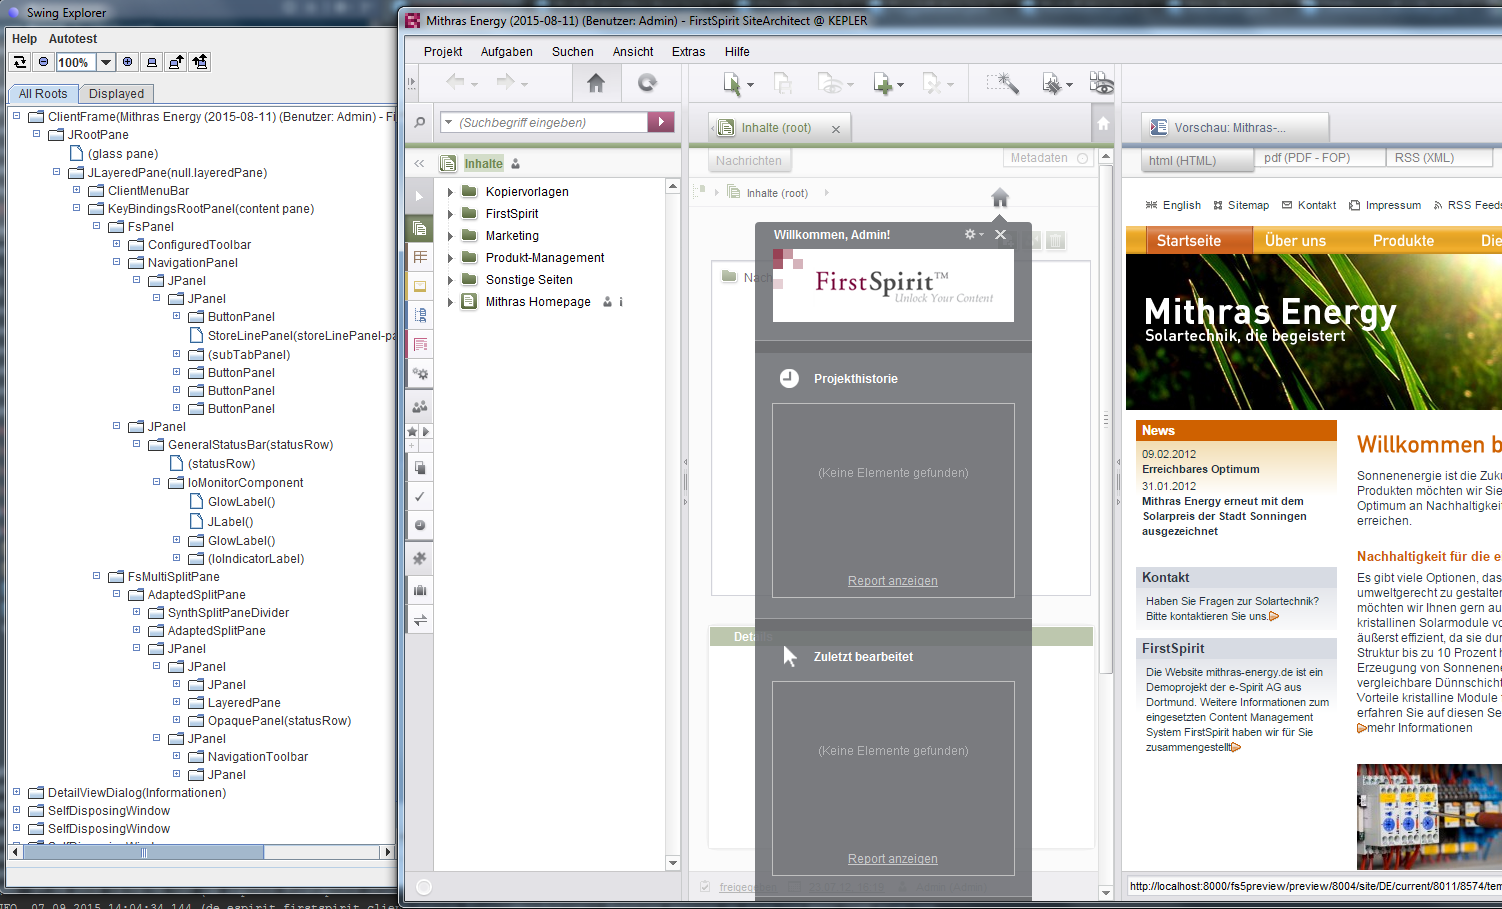
\includegraphics[width=0.85\textwidth]{bilder/screenshot_freespirit.png}
	\caption{Screenshot der e-Spirit CMS-Anwendung FirstSpirit
	sowie anhängigem Swing Explorer, der den Komponentenbaum der Applikation darstellt}
	\label{fig:screenshot_freespirit}
\end{sidewaysfigure}

\begin{figure}
	\centering
	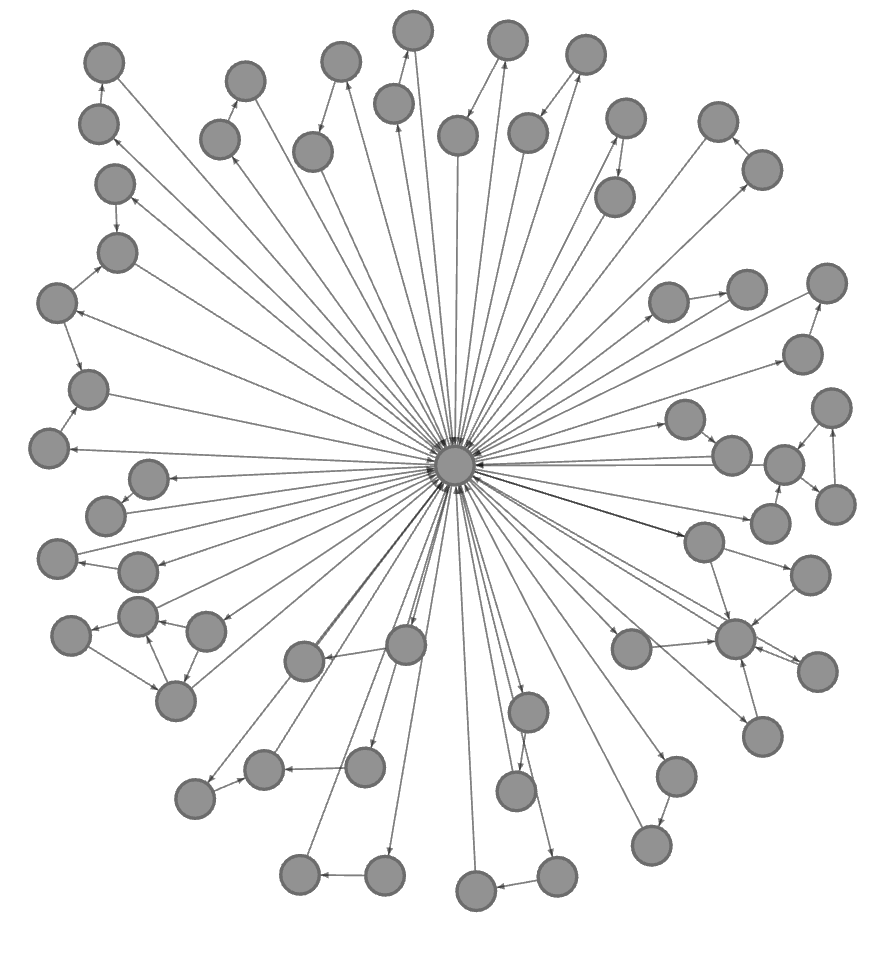
\includegraphics[width=0.85\textwidth]{bilder/model_firstspirit_notext.png}
	\caption{mit Gephi und dem Yifan Hu Algorithmus \cite{hu2005efficient}
    sowie noch für Lesbarkeit maneull angepasste visualierte Graphausgabe 
	des Autotesters über FirstSpirit, hoher Zoomfaktor, keine Beschriftungen.
	Die Pfeile des gerichteten Graphen sind so sichtbar.}
	\label{fig:model_firstspirit_notext}
\end{figure}

\begin{sidewaysfigure}
	\centering
	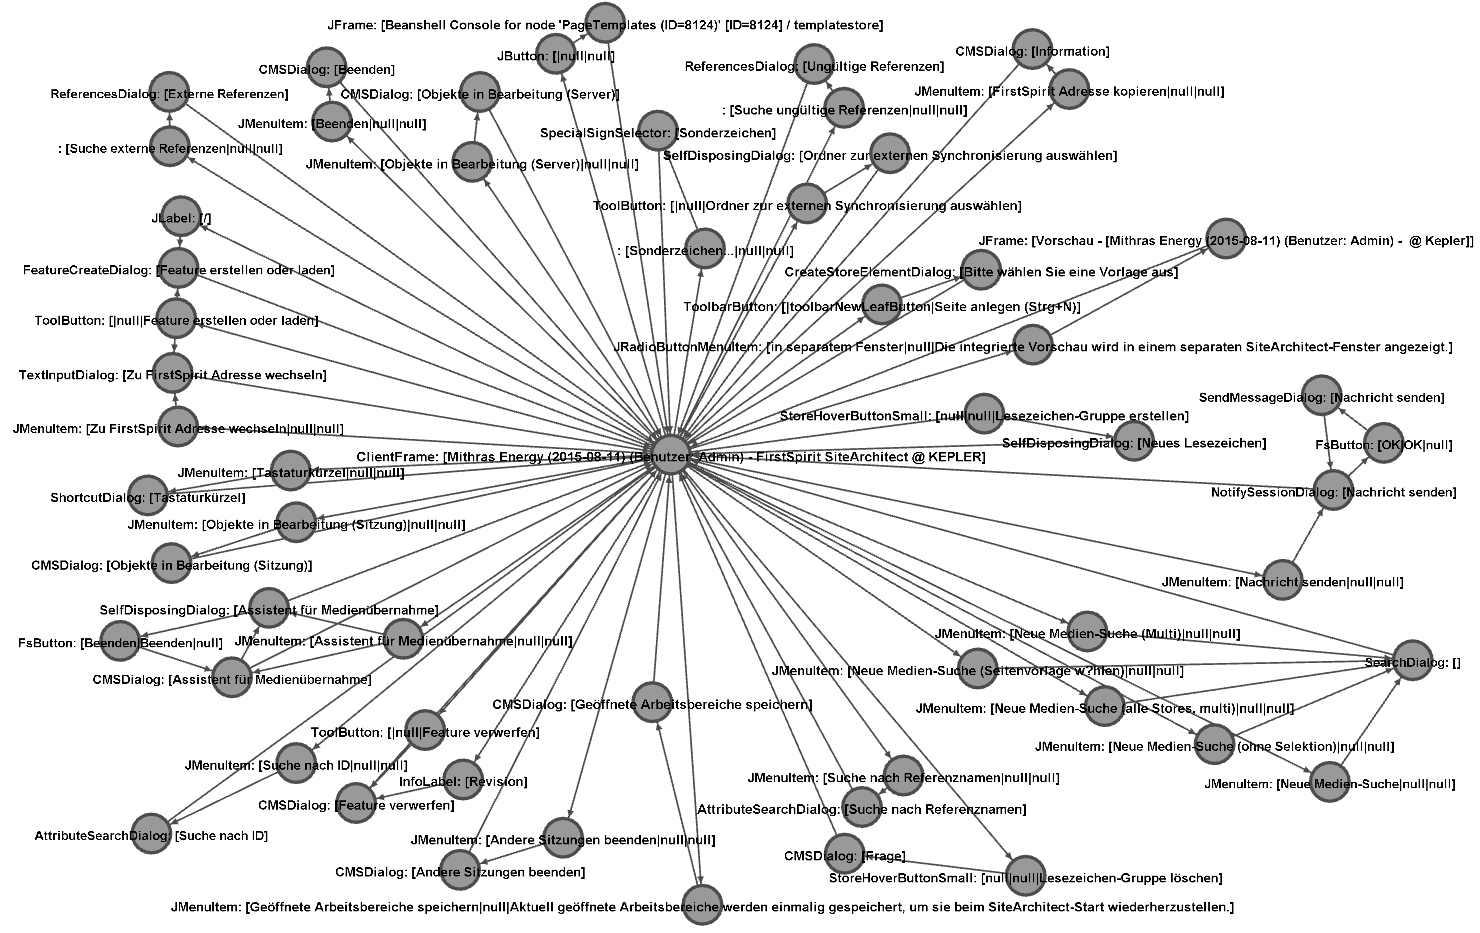
\includegraphics[width=0.85\textwidth]{bilder/model_freespirit.png}
	\caption{mit Gephi und dem Yifan Hu Algorithmus \cite{hu2005efficient}
    sowie noch für Lesbarkeit maneull angepasste visualierte Graphausgabe 
	des Autotesters über FirstSpirit bei einem der ergiebigeren Durchläufe.
	Beschriftungen der Knoten sind aktiviert.}
	\label{fig:model_freespirit_06.10.2015}
\end{sidewaysfigure}



Die Knoten sind in Dreiergruppen angeordnet: Ein Ursprungsfenster, ein Übergangsknoten
(bzw. ein Wort des Modells), sowie der resultierende Zustand bzw. das sich öffnende Fenster.
Dies ist schlicht eine Frage der Lesbarkeit -- anstelle der mittleren Knoten für Übergänge sollten
eigentlich einfach beschriftete Kanten benutzt werden, aber dies schränkt die Möglichkeiten,
den anhängigen Text in eine lesbare Form zu bringen, zu stark ein. Es ist schlicht zu viel
Textinformation, um mit einer Legende o.Ä. auszukommen.

\subsection{Beispiel Fehler FirstSpirit}

FirstSpirit hat eine eigene, robuste Ausnahmebehandlung, die alle Fälle abzudecken
versucht und abgefangene Fehlermeldungen an eine Bugtracker-Schnittstelle bei e-Spirit
weiterleitet. Dennoch gibt es verschiedene Situationen, in denen Ausnahmen erzeugt
und Funktionen unterbrochen werden, die vermutlich besser behandelt werden könnten.
Ein solches Beispiel lautet wie folgt:

\begin{lstlisting}[float=!ht,label=fmjson,caption={Ausnahme bei Eingabe in Suchfeld}]
CreateStoreElementDialog: [Bitte waehlen Sie eine Vorlage aus]
espirit.mpoloczek.CrawlerTester pseudoClickButton
about to pseudo click component FsTextField: []

(de.espirit.firstspirit.client.AbstractGuiHost):
ExceptionHandler.uncaughtException()
java.util.regex.PatternSyntaxException: 
Unclosed character class near index 11
,./;'[]\\-=.*
           ^
at java.util.regex.Pattern.error(Pattern.java:1955)
\end{lstlisting}

Jede Eingabe eines Textes in das Suchfeld hat eine Regex-Muster-Kompilation
zur Folge, unabhängig davon, ob die Eingabe im Sinne von Regex zulässig ist
oder nicht. Es wäre sinnvoller, eine Eingabe zunächst auf Gültigkeit zu prüfen,
anstatt jede zuzulassen bzw. eine Kompilation mit jeder Eingabe zu versuchen.

Ein weiteres Beispiel, diesmal bei einem Datei-Auswahldialog:

\begin{lstlisting}[float=!ht,label=fmjson,caption={Ausnahme bei ungültiger Dateiangabe}]
espirit.mpoloczek.CrawlerTester pseudoClickButton
about to pseudo click component JButton:
[Oeffnen|JFileChooser.ApproveButton|Ausgewaehlte Datei oeffnen]

firstspirit.client.gui.navigation.ppool.sync.FileSystemSyncHandler:
Error accessing directory - java.io.FileNotFoundException:
C:\Users\poloczek\Desktop\<img src or\" '"=alt=javascript:alert(1)\">
\end{lstlisting}

Offensichtlich probierte der Autotester hier einen html-Codeblock als Eingabe eines Dateinamens
aus. Anstatt diese Datei vorher auf Existenz zu überprüfen, versucht FreeSpirit direkt,
die Datei zu öffnen, versagt, und erzeugt diese Ausnahme. Es wäre besser, eine
Eingabe zunächst auf Existenz zu prüfen.


\section{Resultate jEdit}\label{section:testresultsjedit}

Die Wahl für einen zweiten Test fiel auf jEdit
in der neuesten erhältlichen Version 5.3.0,
da der \glqq{}Texteditor für Programmierer\grqq{}
ebenfalls über die benötigte Swing-GUI verfügt und 
durch langjährige Entwicklung bedingt im klassischen
Sinne vermutlich relativ fehlerfrei ist. Eine wenig getestete und daher fehlerträchtige
Applikation ließe keinen vernünftigen Autotest zu, da der Entwickler (oder in diesem Fall
Testentwickler) laufend Probleme bzw. Abstürze im Programm beheben müsste, bis ein vollständiger
Durchlauf und eine Modellbildung möglich wird. Tatsächlich erwies sich jEdit als
dem Testdurchlauf gewachsen -- es wurden zwar nicht abgefangene Ausnahmen produziert,
aber das Programm selbst blieb bei Ausnahmebehandlung durch den Tester lauffähig
und geriet auch in keine Endlosschleifen o.Ä..


\begin{figure}
	\centering
	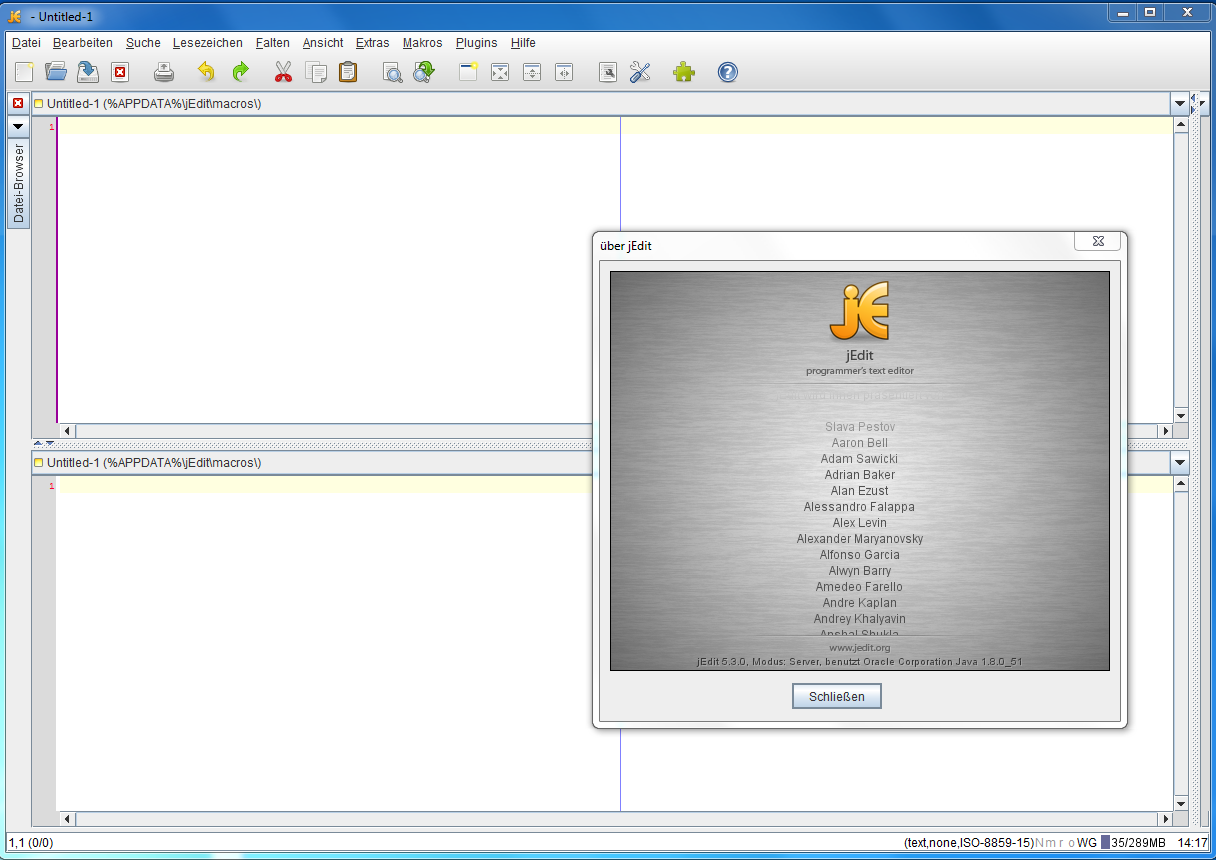
\includegraphics[width=0.85\textwidth]{bilder/jedit_beispiel.png}
	\caption{Screenshot der Java-Applikation jEdit}
	\label{fig:screenshot_jedit}
\end{figure}

\begin{figure}
	\centering
	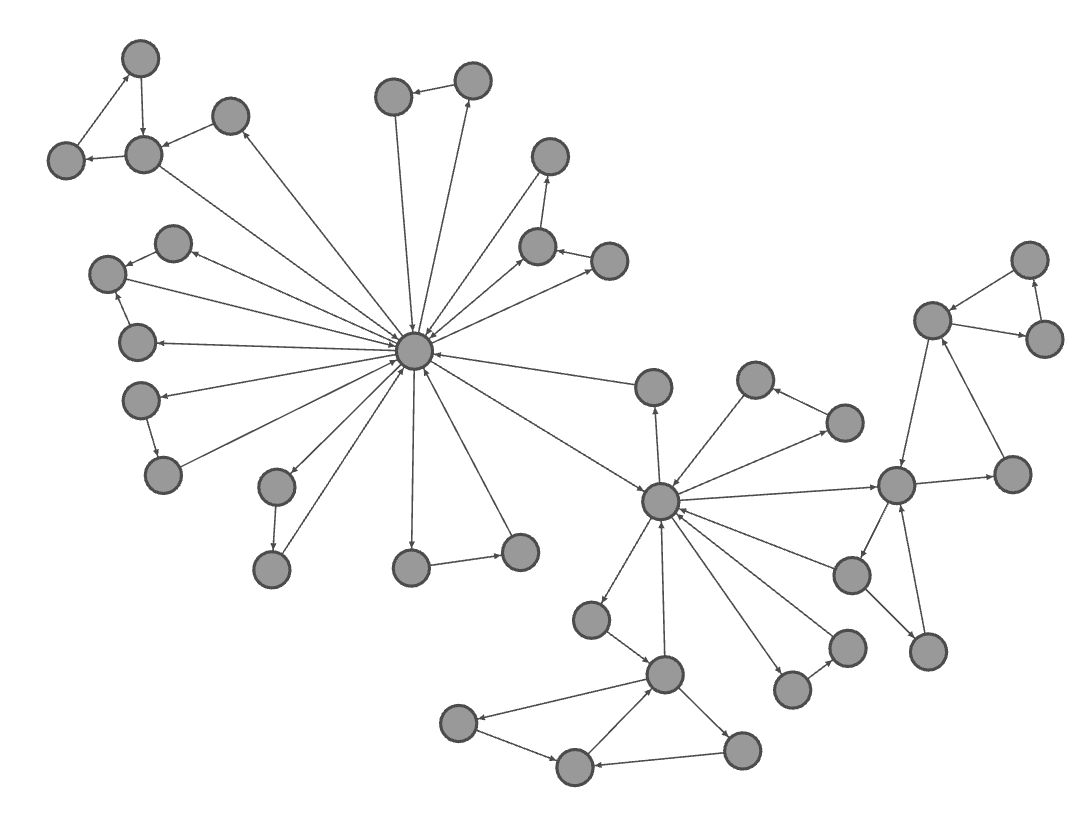
\includegraphics[width=0.85\textwidth]{bilder/model_jedit_notext.png}
	\caption{mit Gephi und dem Yifan Hu Algorithmus\cite{hu2005efficient}
    sowie noch für Lesbarkeit maneull angepasste visualierte Graphausgabe 
	des Autotesters über jEdit, hoher Zoomfaktor, keine Beschriftungen.
	Die Pfeile des gerichteten Graphen sind so sichtbar.}
	\label{fig:model_jedit_notext}
\end{figure}

\begin{sidewaysfigure}
	\centering
	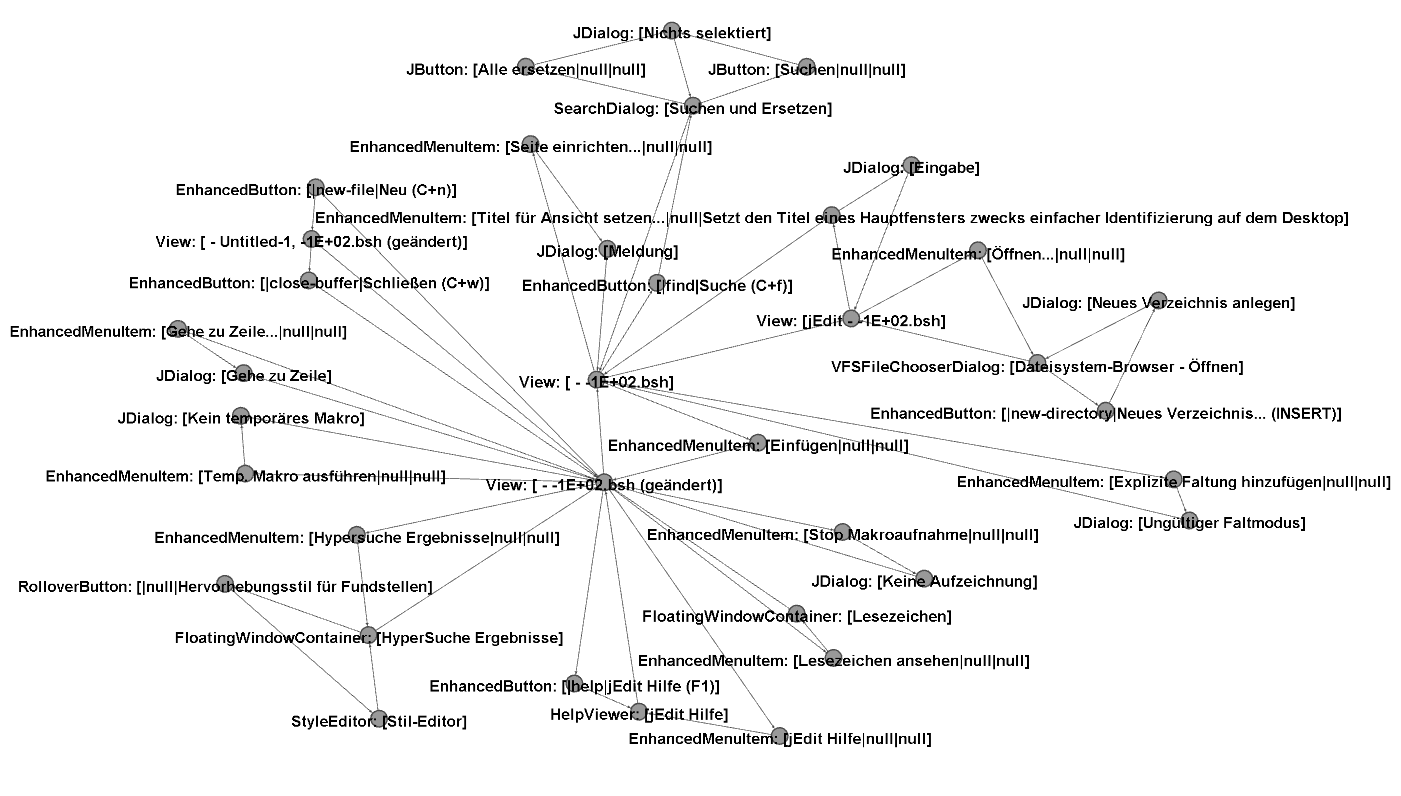
\includegraphics[width=0.85\textwidth]{bilder/model_jedit.png}
	\caption{mit Gephi und dem Fruchterman Reingold Algorithmus\cite{SPE:SPE4380211102}
    sowie noch für Lesbarkeit maneull angepasste visualierte Graphausgabe 
	des Autotesters über jEdit. Beschriftungen der Knoten sind aktiviert.}
	\label{fig:model_jedit}
\end{sidewaysfigure}


Beim Testen von jEdit fielen gewisse Überanpassungen des Autotesters an e-Spirit auf,
welche für eine Entwicklung entlang dieses Programms nicht sonderlich unerwartet
waren. So sah die Konfigurationsdatei beispielsweise nicht vor, Einträge der 
ignorierten Komponenten komplett frei zu lassen. Dies wurde implementiert.
Ebenso fiel auf, dass zwar Zustandsänderungen in Form von sich öffnenden Fenstern
korrekt behandelt wurden, jEdit aber den Zustand des Hauptfensters selbst
ändern kann -- dies würde in FirstSpirit auch passieren, wenn der Tester in der
Lage wäre, das Projekt zu wechseln. (Bei einer unendlich langen Testreihe
wird er dies irgendwann hinbekommen, aber so viel Zeit haben wir nicht)
Der Tester wurde mit Hinblick auf mögliche interne Zustandsänderungen
des aktuell getesteten Fensters erweitert und nimmt dies nun korrekt in
das Modell auf.

Zu sehen ist dies z.B. im Modell von jEdit[\ref{fig:model_jedit}]
auf Seite \pageref{fig:model_jedit} oder im textfreien Fall
[\ref{fig:model_jedit_notext}] auf Seite \pageref{fig:model_jedit_notext}.
Man beachte den sichtbaren Unterschied zu den Modellen von FirstSpirit:
Es existieren gewissermaßen zwei zentrale Zustände anstatt nur einem.
Der zweite Zustand entsteht, weil ein Text in das Editorfeld eingegeben
wurde, wodurch das aktuell geöffnete Dokument in den
\glqq{}[geändert]\grqq{}-Zustand wechselt. Da dieser Zustand
für das Programm selbst vermutlich praktisch überhaupt keine
interne Änderung darstellt, könnte man sie auch als Einen 
gemeinsamen Fall ansehen,
wodurch jEdit eine FirstSpirit stark ähnelnde sternförmige Struktur
aufweisen würde. Dies ist aber aufgrund der baumförmigen
Architektur von Java-Swing und objektorientierter Programmierung
im Allgemeinen, und graphischen Nutzeroberflächen im Besonderen
auch nicht anders zu erwarten. Bei dieser Gelegenheit wurde
der stärkegewichtete 
Fruchterman Reingold Algorithmus\cite{SPE:SPE4380211102}
als Alternative zum bisher verwendeten Yifan Hu\cite{hu2005efficient}
entdeckt. Im Vergleich produziert dieser weniger saubere Trennung
der Knoten, dafür aber eine eckigere Anordnung, die den 
Platzbedürnissen für lesbare Knotenbeschriftungen entgegen kommt.

Weitere neue Herausforderungen stellten sich, als es dem
Autotester gelang, durch zufällige Tasteneingaben ein neues 
Dokument zu erstellen und dies als Druckauftrag 
an den Plotter des Büros zu verschicken. In Folge dieses Vorfalls
hatte der Entwickler reichlich Notizpapier und der Druckerdienst
des betreffenden Arbeitsplatzes wurde vorsorglich deaktiviert.
Ein Auschluss der betreffenden Schaltflächen lässt sich
nur durch nachträgliches Lesen der Logdatei bewerkstelligen.
Dies ist natürlich auch geschehen, aber eine Deaktivierung
der ansonsten ungenutzen Druckfähigkeiten des Rechners
erschien dennoch eine sinnvolle Vorsichtsmaßnahme.

Grundsätzlich gelang dem Autotester auch für jEdit ein
vollständiger Test aller erreichbaren Eingabeelemente
sowie eine Modellierung der zugänglichen Fenster als
Zustände. Es spricht für die Swing-API, dass keine
zusätzliche Erweiterung oder Anpassung der erkundenden
oder Eingaben vornehmenden Algorithmen notwendig wurde.
Eine Ausnahme wurde für die verschiedenen Farbeinstellfelder
des Texteditors gesetzt - jeden einzelnen Knopf in der Farbpallette
auszuprobieren verlängerte den Test erheblich (200 Knöpfe),
und aufgrund der Menüanordnung wurden mehrere Farbpalletten
als separate Zustände aufgefasst. Zwar ist jEdit im Vergleich
zu FirstSpirit wesentlich reaktionsfreudiger -- so kann eine
Pause zwischen Eingaben von 500ms, gerade ein Drittel
des Wertes für den Test von FirstSpirit, gesetzt werden --
überflüssige, da vermutlich stark duplizierende Tests
sind dennoch zu vermeiden.


\subsection{Beispiele für gefundene Probleme jEdit}

Als primärer Texteditor hat jEdit vermutlich robustere Textverarbeitung,
zumindest verglichen mit den anderen Testkandidaten. In der Praxis
hat die Applikation ein der FirstSpirit-Ausnahmebehandlung ähnelndes
Verfahren, welches grundsätzlich jede Ausnahme abfängt und mit einem
Fehlerschirm quittiert, anstatt einen Absturz des Programms zuzulassen.

Dennoch treten noch unbehandelte Ausnahmen auf, wie z.B. die
folgende:

\begin{lstlisting}[float=!ht,label=fmjson,caption={Ausnahme bei Texteingabe}]
about to pseudo click 
component EnhancedMenuItem: [Alle ersetzen|null|null]
[...] Parse error at line 3, column 12.  Encountered: .0
[...] at org.gjt.sp.jedit.bsh.Parser.generateParseException([...])
[...] at org.gjt.sp.jedit.bsh.Parser.jj_consume_token([...])
\end{lstlisting}

Offensichtlich wird auch hier mit Regex oder einem ähnlichen
Symbolverfahren gearbeitet, um ein Suchfeld mit Funktion zu hinterlegen,
und die Eingaben werden vor Kompilation nicht oder nur unzureichend 
auf Zulässigkeit geprüft.

Darüber hinaus fielen nur die üblichen Schwierigkeiten bei der Eingabe
ungültiger Pfade in Datei-Auswahldialogen auf. Diese sind aber zu erwarten
und nicht weiter erwähnenswert. Es gelten die üblichen Empfehlungen,
das Testprogramm sowohl von wichtigen Dateisystemen als auch
der Druckerwarteschlange abzukapseln. Im Verlauf der Tests haben die
automatischen Fehlerberichterstatter den jeweiligen Entwicklern sicher
einige merkwürdig anmutende Logdateien übermittelt.




\section{Resultate yEd}\label{section:testresultsyed}

\begin{figure}
	\centering
	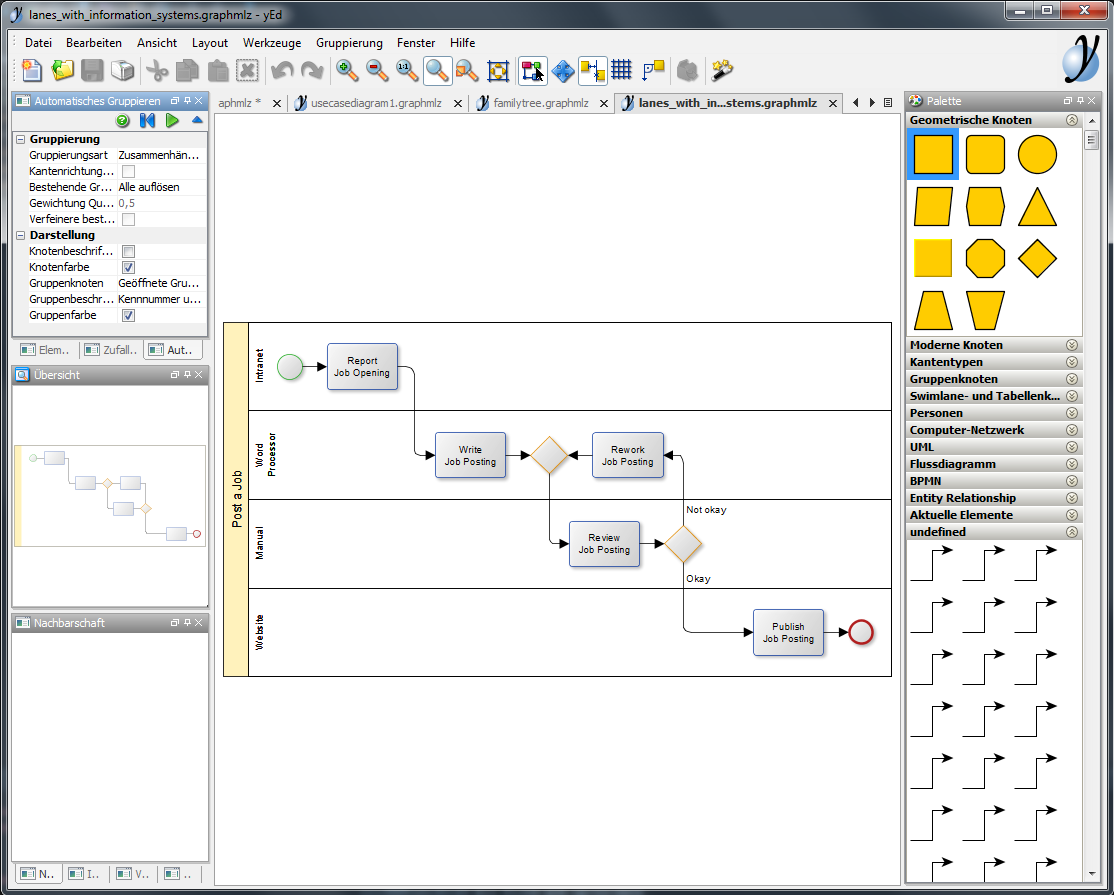
\includegraphics[width=0.85\textwidth]{bilder/screenshot_yed.png}
	\caption{Screenshot yEd während Autotest, man beachte die in Tabs geöffneten, 
	verschiedenen Graphen}
	\label{fig:screenshot_yed}
\end{figure}

\begin{figure}
	\centering
	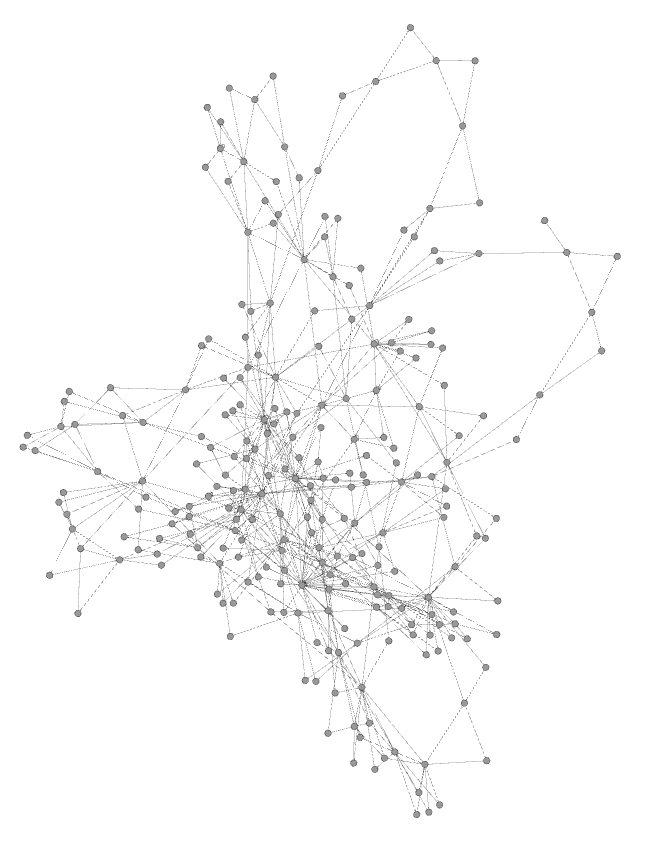
\includegraphics[width=0.85\textwidth]{bilder/model_yed_notext_yh.png}
	\caption{mit Gephi und dem Yifan Hu Algorithmus\cite{hu2005efficient}
    visualierte Graphausgabe des Autotesters über yEd, hoher Zoomfaktor, keine Beschriftungen.}
	\label{fig:screenshot_yed_yh}
\end{figure}

\begin{figure}
	\centering
	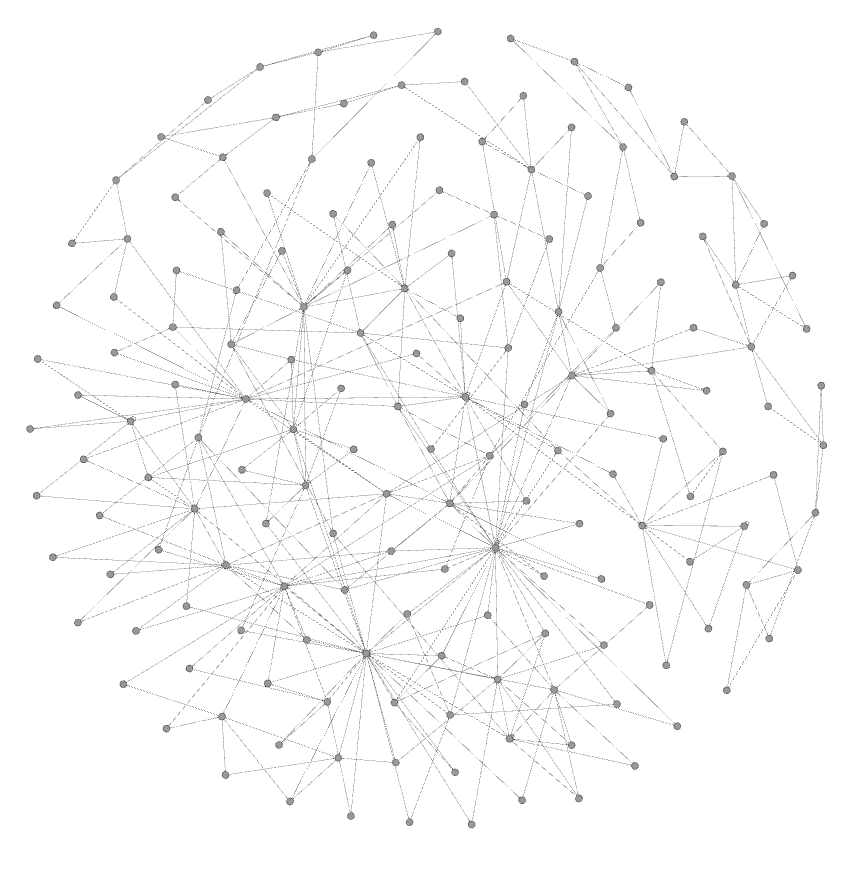
\includegraphics[width=0.85\textwidth]{bilder/model_yed_notext_rf.png}
	\caption{mit Gephi und dem Fruchterman Reingold Algorithmus\cite{SPE:SPE4380211102}
    visualierte Graphausgabe des Autotesters über yEd, hoher Zoomfaktor, keine Beschriftungen.}
	\label{fig:screenshot_yed_rf}
\end{figure}

Als dritte Applikation zum Testen wurde der yEd Graph Editor 
in der aktuellen Version 3.14.4 gewählt,
eine eigenständige Desktopapplikation vergleichbar mit Gephi.
Besonderheiten bezüglich dieses Tests sind z.B., dass yEd Verschleierung
einsetzt, im Englischen Obfuscation genannt. Da die Java-Programmiersprache
Just-In-Time kompiliert wird, enthalten die \glqq{}binären\grqq{}
Dateien noch fast alle Informationen des Quellcodes, und es lässt sich ohne
großen Aufwand äquivalenter Quellcode daraus gewinnen. Dies ist für
Kopierschutz natürlich ein gewaltiges Problem. Im Vergleich dazu lassen
sich auf CPU-Instruktionen kompilierte Programme (sagen wir von C oder C++ aus)
nicht einfach oder eindeutig wieder in Quellcode umwandeln, und der Kompilierer
hat auch die Wahl, sämtliche nutzbaren Meta-Informationen wie Funktionsnamen
zu entfernen.

Eine Lösung dieses Problems für Java ist Obfuscation oder
Verschleierung. Hierbei wird ein Programm zunächst normal kompiliert. 
Danach aber wird vor der Veröffentlichung eine vollautomatische 
Refaktorisierung aller Klassen und Methoden vorgenommen.
Diese hat lediglich zum Ziel, die Bezeichnungen zu ändern. So wird
zum Beispiel aus \glqq{}HauptMenueKlasse\grqq{} schlicht \glqq{}A\grqq{}.
Aus \glqq{}WichtigeFunktion(EingabeKlasse sinnvollerParameterName)\grqq{}
wird \glqq{}a(B a)\grqq{}. Das Resultat ist funktional identisch mit dem
Original, verhält sich also genau gleich, aber eine Begutachtung des
Codes mithilfe eines Dekompilierers ist schwierig bis unmöglich.
Eine kleine Verbesserung der Anwendungsleistung ist ein Nebeneffekt:
Die kürzeren Bezeichnungen sorgen für leicht schnellere Aufrufe, da
kürzere Zeichenketten verglichen werden müssen.

Für den Autotester hat Verschleierung keinerlei Bedeutung, da Aufrufe
an die Swing-API (oder Systemaufrufe oder Aufrufe an nicht verschleierte 
Bibliotheken) nicht versteckt werden können. Oder: So lange ein Programm
lauffähig ist, ist es maschinell auch lesbar. Die zur Identifikation von Komponenten
benutzten Informationen wie Fenstertitel lassen sich ebenfalls nicht verschleiern,
ohne den Nutzen der Anwendung zu zerstören. Was dem Autotester eher
zu schaffen macht, ist die erhebliche Komplexität des Programms und
insbesondere auch die vielen Beispielprojekte, die über Schaltflächen
zugänglich sind. Seiner Natur entsprechend, probiert der Tester diese
natürlich alle aus, was in Änderungen des Hauptfensters resultiert, was
weitere Tests nach sich zieht etc. Betrachtet man die visualisierten
Ausgaben des Zustandsgraphen \ref{fig:screenshot_yed_yh} und 
\ref{fig:screenshot_yed_rf}  auf Seiten \pageref{fig:screenshot_yed_yh} 
und \pageref{fig:screenshot_yed_rf}, sieht man den Unterschied zu vorherigen
Anwendungen sofort. Der Graph erscheint verteilt, ohne klares Zentrum
oder Ursprungspunkt. Dies liegt an den Beispielprojekten, die praktisch
eigene Mini-Ursprungspunkte darstellen. Daraus folgen fast 1700
Eingabeelemente und 74 Fenster, die vom Autotester durchsucht
bzw. ausprobiert werden mussten. Erschwerend kam noch hinzu,
dass eine Sprachumschaltung enthalten ist, welche die Metainformationen
verändert, auf denen die Graphbildung aufbaut. Fenstertitel
unterscheiden sich im deutschen und englischen Modus voneinander.


\subsection{Beispiele für gefundene Probleme yEd}

Nachdem durch iterative Erweiterung der Bannlisten/Blacklists
ein vollständiger Durchlauf des Autotesters über yEd erreicht wurde,
konnte damit begonnen werden, die Logdateien auf Fehler zu
durchsuchen. yEd verfügt über eine integrierte Ausnahmebehandlung,
die jeden Absturz zu verhindern sucht. Anstattdessen öffnet yEd eine
Fehlermeldung, was sehr löblich ist, aber im Vergleich zu FirstSpirit
nicht ideal. Dieses meldet Ausnahmen nur im Hintergrund und leitet
diese automatisch an den Online-Bugtracker von e-Spirit weiter,
sodass die Entwickler sich darum kümmern können und auch gleich
Statistiken darüber bekommen, welche Fehler wie häufig auftraten.
Es gelingt dem Autotester auch hier, unvollständige Fallabdeckung
und sogar zumindest ein kritisches Problem aufzudecken.

Als erstes Beispiel diene der schlichte Fall unerwarteter Zeichenketten:

\begin{lstlisting}[float=!ht,label=fmjson,caption={Ausnahme bei Eingabe einer Nicht-Zahl}]
java.lang.NumberFormatException: For input string: "<a"
at java.lang.NumberFormatException.forInputString[...]
at java.lang.Integer.parseInt(Integer.java:580)
at java.lang.Integer.parseInt(Integer.java:615)
at y.E.R.?(Unknown Source)
at y.E.R.?(Unknown Source)
at y.E.uA$A.setText(Unknown Source)
at espirit.mpoloczek.CrawlerTester$EDTCompliantTextSetter.run[...]
\end{lstlisting}

Die Applikation erzeugt eine unbehandelte Ausnahme, wenn in einem
Textfeld etwas eingegeben wird, das keine Zahl ist. Die korrekte Behandlung
einer solchen Situation wäre das Abschalten des entsprechenden Eingabeelements,
bis eine korrekte Eingabe erfolgt. Dies ist eine der häufigsten Fehlerquellen,
die vom Autotester aufgedeckt werden. Aufgrund der Verschleierung von
yEd ist es nur dem Entwickler selbst (hoffentlich) möglich, zu sagen,
was genau \glqq{}y.E.uA\$A\grqq{} ist und wie dieser Fehler im Quellcode
zu beheben wäre.

Als zweiter Fund dient die Schaltfläche \glqq{}Knotenüberlappungen auflösen\grqq{}.
Zum Zeitpunkt dieser Eingabe war eines der Beispiel-Graph-Projekte geöffnet.
Aus dem folgenden Abschnitt der Logdatei geht hervor, dass nach Betätigung
dieser Schaltfläche mindestens zehn Sekunden lang gar nichts mehr geschah,
der Autotester also darauf wartete, den Kontrollfluss von der Implementation der
Schaltfläche wieder zurückzuerhalten, während yEd irgendetwas tat. Der
folgende Fehler \glqq{}OutOfMemoryError: Java heap space\grqq{}
deutet auf einen Programmierfehler in yEd hin, der zu einer Endlossschleife
bis hin zum Absturz der Java Virtual Machine führt. Die Applikation \glqq{}hängt\grqq{}, bis
dieser Absturz erfolgt. Leider verfügt die Logdatei des Autotesters nicht über einen
detaillierten Kontext (woher auch), aber dies stellt einen schweren Fehler in yEd
dar und sollte baldmöglichst behoben werden.

\begin{lstlisting}[float=!ht,label=fmjson,caption={Ausnahme yEd durch Schaltfläche \glqq{}Knotenüberlappungen auflösen\grqq{}}]
espirit.mpoloczek.CrawlerTester pseudoClickButton
about to pseudo click component JMenuItem: [Knotenueberlappungen ...]
espirit.mpoloczek.CrawlerTester$TimerRunner run
No actions were taken for 10 seconds, deadlock situation??
---> BEGIN ERROR
java.lang.OutOfMemoryError: Java heap space
at com.sun.java.help.search.Query.makePenaltiesTable[...]
at com.sun.java.help.search.Query.<init>(Query.java:43)
at com.sun.java.help.search.Search.<init>(Search.java:51)
at com.sun.java.help.search.QueryEngine.processQuery[...]
at com.sun.java.help.search.DefaultSearchQuery.run[...]
at java.lang.Thread.run(Thread.java:745)
---> END ERROR
\end{lstlisting}



\section{Vergleich mit klassischen Tests}\label{section:testcomparisonclassic}

Ein Vergleich mit halbautomatischen Methoden oder gewöhnlichen Unit-Tests
ist erst einmal schwierig, da diese auf anderen Prinzipien aufbauen.
Üblicherweise ist das Ziel die Überprüfung der Korrektheit des Programms.
Um eine Aussage über Korrektheit treffen zu können, sind kontextuelle
Informationen über ein Programm bzw. das gewünschte Verhalten notwendig.
Einem vollautomatischen Ansatz stehen diese Informationen schlicht nicht
zur Verfügung. Das hier vorgestellte Konzept ist auch nicht als Ersatz 
klassischer Tests gedacht oder in irgendeiner Form äquivalent.

Getreu dem Zitat von Dijkstra \footnote{ACM Turing Lecture 1972},
nach dem die Abwesenheit von Fehlern nicht bewiesen werden kann,
zielt der Autotester in eine andere Richtung. Es wird versucht, so viele
unerwartete Situationen und resultierende Fehler zu erzeugen, wie
irgendwie möglich. Man kann ihn also als ein Komplement bzw. eine Addition
zu klassischen Tests verstehen bzw. Einsetzen.

Ein Durchlauf des Autotesters ist verglichen mit Unit Tests und den
meisten Regressionstests eher langsam. Ein vollständiger Durchlauf
über FirstSpirit dauert ungefähr 20 Minuten. Leider gibt es für die
Emulation menschlicher Eingaben und der Wartezeit für die Verarbeitung
dieser Eingaben durch das Programm keine guten Alternativen.
Man bedenke allerdings: Derselbe Test durch einen Menschen würde
noch erheblich länger dauern und die üblichen menschlichen Fehlerquellen
beinhalten, die das Ergebnis zusätzlich beeinflussen. Auch handelt es
sich bei der Entwicklerversion von FirstSpirit um ein massives
Konstrukt mit Serverbedingt behäbigen Reaktionszeiten und gewaltigem
Funktionsumfang, also vielen (beinahe eintausend) zu testenden Elementen.

Auch wurden im Verlauf dieser Arbeit nur relativ alte und bewährte
Applikationen getestet, welche auf jahrelange Entwicklung und Nutzung
zurückblicken können und daher auch selbst unwahrscheinliche
Fehlerquellen bereits erlebt und behoben haben. Unzuverlässige
Applikationen der Java-Swing Schnittstelle sind längst in Vergessenheit
geraten.

Das Konzept an sich wäre aber insbesondere in den Anfangsphasen
eines Projekts von besonderem Wert, wenn nur Entwickler daran
arbeiten und noch keine Tester beteiligt werden bzw. noch nicht
genug Funktionalität vorliegt, um sinnvoll zu testen. Explorative,
destruktive Eingaben sind immer möglich, wenn überhaupt
Eingaben getätigt werden können. Mit dem Autotester können
sehr schnell unvorhergesehene Situationen herbeigeführt
und noch in der Entwicklungsumgebung analysiert und evtl.
behoben werden.
